\section{Exemplo de uso BBN}

Considere o caso de um carro que possui a funcionalidade de abaixar os vidros por um comando pela chave. A rede apresentada na figura \ref{fig:bateria1}, modela como o estado da bateria da chave e da bateria do carro podem influenciar em ações apreciáveis, como ligar o carro e abaixar a janela. 

Nesse caso, a bateria do carro e a bateria da chave são variáveis que influenciam diretamente o estado de abaixar a janela do carro, enquanto a ação de ligar o carro depende apenas do estado da bateria do carro. Nesse caso, a inexistência de uma "seta" entre a bateria do carro e a ação de ligar o carro indica esta independência.


\begin{figure}[H]
  \centering
  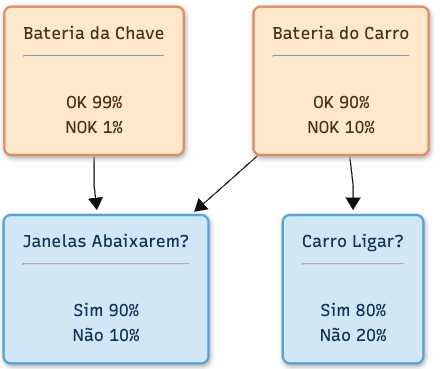
\includegraphics[width=0.5\textwidth]{Cap3/BateriaCarro1.png}
  \caption{Rede Bayesiana para o sistema de controle do carro.}
  \label{fig:bateria1}
\end{figure}

Agora, considere o caso em que, apertando a chave, o carro abre, porém, não abaixa a janela. Nesse caso, a rede apresentada na figura \ref{fig:bateria2} modela como essa atualização (o não abaixar da janela) altera as probabilidades de ligar o carro e a probabilidade da bateria do carro estar descarregada.

\begin{figure}[H]
  \centering
  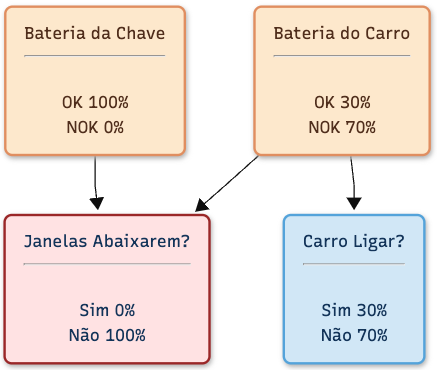
\includegraphics[width=0.5\textwidth]{Cap3/BateriaCarro2.png}
  \caption{Rede Bayesiana para o sistema de controle do carro, tendo observado o estado da bateria da chave e a ação das janelas.}
  \label{fig:bateria2}
\end{figure}

Este é um exemplo prático de como as CTPs de uma BBN se alteram com a observação de variáveis. No cenário em que a ação de ligar o carro é, na verdade, um teste de lançamento de foguete extremamente caro, a observação de uma variável inicialmente não correlacionada e a utilização de uma BBN bem alimentada poderia indicar que o teste não deveria ocorrer, economizando recursos e evitando riscos desnecessários.
